\documentclass{article} %[twocolumn]

\usepackage{algorithmicx}
\usepackage{algpseudocode}
\usepackage{booktabs}
\usepackage{array}
\usepackage{graphicx}
\usepackage{amsmath}
\usepackage{amsfonts}
\usepackage{textcomp}
\usepackage{multirow}
\usepackage{subfig}

\DeclareMathOperator*{\argmax}{arg\,max} 

\title{Bayesian design of pilot trials for complex interventions}

\begin{document}

\maketitle

\begin{abstract}
\textbf{Background}: 
\textbf{Methods}: 
\textbf{Illustration}: 
\textbf{Conclusions}: 
\end{abstract}

\section{Introduction}\label{sec:introduction}

External pilot trials are a common component of the complex intervention development and evaluation pathway~\cite{Craig2008}. They are used to gather information regarding the feasibility and design of a larger, confirmatory trial of the intervention. Some common aims of pilot trials include the assessment of recruitment rates, data completeness, adherence to interventions, and compliance with randomisation~\cite{Avery2017}. They generally take a similar form to the planned confirmatory trial, although with a significantly reduced sample size~\cite{Eldridge2016}.

Formal statistical approaches to the design and analysis of pilot trials are not commonly used. The sample size is often chosen using a simple rule-of-thumb, such as recruiting at least 30 participants to each arm~\cite{Lancaster2004, Browne1995}\footnote{As previously discussed, this rule seems to have been born out of a mis-reading of the Browne paper - he actually advised against using this rule-of-thumb.}. Although hypothesis testing has been advised against due to concerns about underpowered analyses~\cite{Lancaster2004, Arain2010}, pre-specified progression criteria are often used to determine whether a confirmatory trials should be undertaken and, if so, whether any modification to the intervention or the trial design should be undertaken to ensure its feasibility. These progression criteria specify thresholds against which a parameter estimate is to be compared. For example, consider a pilot trial which will estimate the probability that a participant will be lost to follow-up, $\hat{p}$. An associated progression criteria could be: if $\hat{p} > 0.35$, do not proceed; if $\hat{p} < 0.25$; and if $0.25 < \hat{p} < 0.35$, proceed but only after making modifications to the intervention or trial design aimed at improving data collection. 

Despite the critical role progression criteria play in decision making, there is relatively little methodological guidance regarding how they should be determined~\cite{Avery2017}. If poor criteria are used, the probability of making an incorrect decision may be unacceptably high. A more formal approach to choosing progression criteria, involving statistical analysis of the probability of making such incorrect decisions, may help avoid this. However, such an approach will incur a number of statistical challenges~\cite{Wilson2015}. Multiple outcomes must be considered, data will often be of a multilevel nature due to cluster randomisation or clustering due to treatment provision, the sample size will necessarily be small, and there may be significant uncertainty regarding the value of nuisance parameters (e.g. the ICC in a clsuetr randomised trial~\cite{Eldridge2015}). In this paper we will develop and illustrate a method which can overcome each of these challenges. We propose a Bayesian approach, allowing  for any external information or knowledge to be formally incorporated, and uncertainty in nuisance parameters to be fully expressed, via prior distributions.

The remainder of this paper is organised as follows. A motivating example of a pilot trial in a care home setting is introduced in Section~\ref{sec:motivating example}. The methodology, including details on design optimisation, is then described in Section~\ref{sec:methods}. We illustrate the proposed approach in Section~\ref{sec:illustration}, before discussing implications and limitations in Section~\ref{sec:discussion}.

\section{Motivating example}\label{sec:motivating example}

The REACH (Research Exploring Physical Activity in Care Homes) trial~\cite{Forster2017} aims to inform the feasibility and design of a future definitive RCT assessing a complex intervention designed to increase the physical activity of care home residents. The trial is cluster randomised due to the whole-home nature of the intervention, which is designed to assist care-home staff to make step-by-step changes in their approach to working with residents.

The trial will collect data pertaining to the recruitment of care home residents to the trial, the successful delivery of the intervention, the completeness of follow-up data collection, and the effectiveness of the intervention.

[TO COMPLETE]

\section{Methods}\label{sec:methods}

\subsection{Design and analysis}\label{sec:specification}

Consider a pilot trial which will produce data $x$ according to model $p(x | \theta)$. We assume the design of the trial, including its sample size, is known and fixed. The parameters of substantive interest are denoted by $\phi$, nuisance parameters by $\psi$, with $\theta = (\phi, \psi)$. We assume that a joint prior distribution $p(\theta)$ has been specified. We do not impose any particular restrictions regarding the form of the model or the prior distribution, other than that samples from the prior and the posterior $p(\theta | x)$ can be generated.

Following the observation of the pilot data $x$, a decision must be made regarding whether or not to progress to a confirmatory RCT. Following the convention in pilot trials, we consider three possible actions. We may: discard the intervention and stop all future development or evaluation; proceed immediately to a confirmatory RCT; or proceed to a confirmatory RCT, but only after some modifications to the intervention, the planned trial design, or both, have been made. We denote these decisions as $r$(ed), $g$(reen) and $a$(mber) respectively. We make two assumptions regarding our preferences amongst these three decisions. Specifically, for any $i, j \in \{r, a, g\} = \mathcal{D}, i \neq j,$
\begin{enumerate}
\item Our preference between $i$ and $j$, given $\phi$, is independent of $\psi$;
\item For any $\phi$, either $i$ is strictly preferred to $j$, or vice versa.
\end{enumerate}
Assumption (1) formalises the separation of $\theta$ into substantive and nuisance components, while assumption (2) guarantees the existence of a unique optimal decision. We denote by $\Phi_{I}$ the set of substantive parameter values for which decision $i$ is preferred to the alternatives, $\Phi_{I} = \{ \phi \in \Phi \mid i \succ j ~\forall ~j \in \mathcal{D} \}$. By assumption (2) the entire substantive parameter space is partitioned as $\Phi = \Phi_{R} \cup \Phi_{A} \cup \Phi_{G}$. We will henceforth refer to these three subsets as \emph{hypotheses}. Throughout, we will distinguish hypothesis $I$ from the corresponding decision $i$ by using capital and lower case letters respectively.

Given the observed data $x$ a decision is made by first calculating the marginal posterior probabilities
\begin{align}
p_{R} & = Pr[\phi \in \Phi_{R} \mid x] \\
p_{G} & = Pr[\phi \in \Phi_{G} \mid x].
\end{align}
Note that $p_{A} = 1 - p_{R} - p_{G}$, and that $(p_{R}, p_{G}) \in \{[0,1]^{2} \mid 0 \leq p_{R} + p_{G} \leq 1 \} = \mathcal{P}$. A decision rule $a_{\delta}(p_{R}, p_{G}): \mathcal{P} \rightarrow \mathcal{D}$ is then applied.  The rules we consider  partition the posterior probability space $\mathcal{P}$ into exactly three subsets corresponding to the three decisions, are are parametrised by defined by parameter $\delta = (\delta_{1} , \ldots , \delta_{4}) \in [0,1]^{2} \times [0, \pi]^{2} = \Delta$ as illustrated in Figure~\ref{fig:rule_simple}. The boundary between red and amber regions is a straight line intercepting the $y$-axis at $\delta_{1}$ at an angle of $\delta_{3}$. Similarly, the boundary between amber and green regions is a straight line intercepting the $x$-axis at $\delta_{2}$ at an angle of $\delta_{4}$. A rule is considered valid only if it prevents decision $i$ from being made when the posterior probability of hypothesis $\Phi_{I}$ is zero; and if the intersection of the two boundary lines (shown as a cross in Figure~\ref{fig:rule_simple}) is not in the interior of $\mathcal{P}$. The latter condition ensures that the red and green regions are never adjacent. We assume that the decision rule has been specified in advance, and will discuss how it may be chosen in Section~\ref{sec:optimisation}. 

\begin{figure}
\centering
\includegraphics[scale=0.7]{./Figures/dr_ex_simple}
\caption{Example decision rule.}
\label{fig:rule_simple}
\end{figure}

\subsection{Evaluation}\label{sec:evaluation}

Given a proposed pilot trial design and associated model, a prior distribution for the parameters of the model, and a decision rule, we wish to define some appropriate operating characteristics which can be used to evaluate and compare different designs. We propose that three events are of particular interest, and define the operating characteristics as their unconditional probabilities. Specifically, we consider the probability of: running a futile confirmatory trial ($OC_{1}$); making unnecessary adjustments to the trial design or the intervention ($OC_{2}$); and discarding a promising intervention ($OC_{3}$). Each of these can be specified in terms of the probabilities of making decision $j$ when $\phi \in \Phi_{I}$, as set out in Table~\ref{tab:probs}:

\begin{table}
\centering
\begin{tabular}{r r r r r r}
\toprule
& & \multicolumn{3}{c}{Truth} & \\
& & $R$ & $A$ & $G$ & \\
\midrule
\multirow{3}{*}{Decision} & $r$ & $p_{R,r}$ & $p_{A,r}$ & $p_{G,r}$ & $A_{r}$ \\
 & $a$ & $p_{R,a}$ & $p_{A,a}$ & $p_{G,a}$ & $A_{a}$ \\
 & $g$ & $p_{R,g}$ & $p_{A,g}$ & $p_{G,g}$ & $A_{g}$ \\
 \midrule
 & & $\Phi_{R}$ & $\Phi_{A}$ & $\Phi_{G}$ & 1 \\
\bottomrule
\end{tabular}
\caption{Probabilities of decisions and hypotheses.}
\label{tab:probs}
\end{table}

\begin{enumerate}
\item $OC_{1}$ - running a futile confirmatory trial ($p_{R,a} + p_{R,g} + p_{A,g}$);
\item $OC_{2}$ - making unnecessary adjustments ($p_{R,a} + p_{G,a}$);
\item $OC_{3}$ - discarding a promising intervention ($p_{A,r} + p_{G,r} + p_{A,g}$).
\end{enumerate}
The probability of making decision $j$ when $\phi \in \Phi_{I}$ is
\begin{equation}
p_{I,j} = \mathbb{E}_{\theta} [ \mathbb{I}(\phi \in \Phi_{I} ~\&~ a_{\delta}(p_{R}, p_{G}) = j) ],
\end{equation}
where the expectation is with respect to the prior distribution $p(\theta)$ and $\mathbb{I}(.)$ is the indicator function. We can compute Monte Carlo estimates of these probabilities by sampling $\theta^{(1)}, \ldots , \theta^{(N)}$ from the prior distribution $p(\theta)$, from which we extract $\phi^{(1)}, \ldots , \phi^{(N)}$. For each $\theta^{(k)}$, data $x^{(k)} \sim p(x | \theta^{(k)})$ is then simulated. A Bayesian analysis is conducted, from which the posterior probabilities $p_{R}^{(k)}, p_{G}^{(k)}$ are extracted. We then have
\begin{equation} \label{eqn:MC_prob}
p_{i,j} \approx \frac{1}{N} \sum_{k=1}^{N} \mathbb{I}(\phi^{(k)} \in \Phi_{I}, a(p_{R}^{(k)}, p_{G}^{(k)}) = j).
\end{equation}

When (MC)MC methods are required to perform the Bayesian analysis the posterior probability $p_{R}^{(k)}$ (likewise $p_{G}^{(k)}$) is itself a Monte Carlo estimate, based on $M$ samples $\phi^{(m)}$ from the marginal posterior distribution $p(\phi | x^{(k)})$. Specifically,
\begin{align}
p_{R}^{(k)} &= \mathbb{E}_{\phi \mid x^{(k)}} [ \mathbb{I}(\phi \in \Phi_{R}) ] \\
 & \approx \frac{1}{M} \sum_{m=1}^{M} \mathbb{I}(\phi^{(m)} \in \Phi_{R}).
\end{align}
We assume that $M$ MCMC samples will be used when calculating the posterior probabilities $p_{R}, p_{G}$ given the actual observed pilot data, and thus that the process being simulated corresponds exactly to that which will be carried out in practice. Any error in the estimation of $p_{I,j}$ therefore stems only from the finite number of samples used in the outer loop, $N$. For large $N$ the error of the unbiased MC estimate of any probability $p$, including each of the operating characteristics, will be normally distributed with variance approximately equal to $p(1-p)/N$.

%Estimating trial operating characteristics through this nested MC scheme is conceptually simple, but suffers from two difficulties. Firstly, the large number of MCMC analyses to be carried out ($N$) prohibits the usual visual assessment of chain convergence. Secondly, the computational burden is significant, requiring $N \times M$ samples in total to be generated. 

\subsection{Optimisation}\label{sec:optimisation}

Evaluation of a trial design is computationally expensive, requiring the generation of $N \times M$ samples. If any changes are made to the sample size of the design, the entire process must be repeated. However, if changes are only made to the decision rule, the same set of $N$ simulated data sets and corresponding Bayesian inferences can be re-used when evaluating the new design. This suggests that, for a fixed sample size, optimisation over the possible decision rules could find that which delivers the best operating characteristics.

Recall from Section~\ref{sec:specification} that $\Delta$ is the space of all decision rules. We wish to find the $\delta \in \Delta$ which minimises the operating characteristics $OC_{i}(\delta)$, $i= 1,2,3$. Note, however, that these will typically be in conflict in the sense that any decrease in one will be accompanied by an increase in another. As such, there is no single optimal decsiion rule. However, we can use the notion of Pareto dominance to compare any two rules and identify if one is superior to the other. Formally, we say that rule $\delta_{*}$ dominates $\delta$, denoted $\delta_{*} \prec \delta$, if $OC_{i}(\delta_{*}) \leq OC_{i}(\delta) ~ \forall ~ i$ and $OC_{j}(\delta_{*}) < OC_{j}(\delta)$ for some specific $j$. In this case, rule $\delta_{*}$ should always be preferred to rule $\delta$ because it is at least as good in all respects, and strictly better in at least one. We can then define the \emph{Pareto set} as the set of rules which are not dominated by any other rule. Ideally the optimisation procedure would return the Pareto set, but in practice we will find some approximation of it. 

An \emph{approximation set} $\mathcal{A}$ is a set of rules which are not dominated by any other rule in $\mathcal{A}$~\cite{Emmerich2011}. Optimising over the space of decision rules aims to find an approximation set $\mathcal{A}$ which is as close as possible to the Pareto set. Clearly, we wish for $\mathcal{A}$ to contain rules which lead to operating characteristics close to those obtained by the Pareto set. However, $\mathcal{A}$ should also provide a sufficient range of options regarding the balance between the three operating characteristics. In this way, the decision maker can view the approximation set, assess the relative trade-offs between the three operating characteristics which are available, and choose the decision rule which best reflects their priorities. An illustration of a Pareto set and two approximation sets is given in Figure~\ref{fig:pareto_example}, where we have considered only operating characteristics $OC_{1}$ and $OC_{3}$. Approximation set $\mathcal{A}_{2}$ contains only three rules, although these are all of high quality in terms of both operating characteristics, being close to the Pareto set. However, the larger number of rules in set $\mathcal{A}_{2}$ provides more opportunity for the decision-maker to select a rule which balances their priorities.

\begin{figure}
\centering
\includegraphics[scale=0.7]{./Figures/pareto_example}
\caption{Example Pareto and approximation sets.}
\label{fig:pareto_example}
\end{figure}

An approximation set can be obtained by applying a multi-objective optimisation algorithm such as the benchmark algorithm NSGA-II~\cite{Deb2002}, as implemented in the R package~\cite{Mersmann2014}. 

\subsection{Utility}

Recall that the analysis of the trial will come down to computing the three posterior probabilities $Pr[\phi \in \Phi_{i} | x]$. When making a decision based on these summaries, we are concerned with balancing the costs of each type of error and the probabilities that these will be made. If we assign a fixed cost to our three errors, $c_{1}, c_{2}$ and $c_{3}$, we can define a loss function which will take the following values: 

\begin{table}
\centering
\begin{tabular}{r r c c c}
\toprule
& & \multicolumn{3}{c}{Truth} \\
& & $R$ & $A$ & $G$ \\
\midrule
\multirow{3}{*}{Decision} & $r$ & 0 & $c_{2}$ & $c_{2}$ \\
 & $a$ & $c_{1} + c_{3}$ & 0 & $c_{3}$ \\
 & $g$ & $c_{1}$ & $c_{1} + c_{2}$ & 0  \\
\bottomrule
\end{tabular}
\caption{Loss function values.}
\label{tab:probs}
\end{table}

Now, assuming that this loss function has been defined in the proper manner and accounts for attitude to risk, we know that the best decsion is that which minimises the posterior loss. That is, we would choose
\begin{equation}
d = \arg\min_{d \in \{r,a,g\}} \mathbb{E}_{\phi | x} [ L(d, \phi) ].
\end{equation}
Note that this can be translated into a rule based on posterior probabilities as previously discussed, but that this formulation has less parameters. In fact, since loss is invariant under a linear transformation, the costs parameters can be scaled so $c_{1} + c_{2} + c_{3} = 1$ and thus only two parameters must be chosen (compared with 4 in the previous model). 

What assumptions have we encoded in using a loss function of this form? We can consider the problem as one of three binary attributes - for each type of error, either it is made or it isn't. We have then assumed that the losses of each attribute are additive - the cost of making one type of error is not affected by whether or not we are making another type of error also. Since each attribute is binary, there is no scope or need to consider attitude to risk separately to the value of a deterministic outcome. How can we validate/verify the function? The parameters will imply the equivalence of a set of gambles. For example, suppose $c_{1} = 0.5, c_{2} = 0.4$ and $c_{3} = 0.1$. Then we must be unable to choose between gamble A: type I error with probability 0.5, or no error with probability 0.5; and gamble B: a type II with probability 0.375, and a type III error with probability 0.625 [they both give an expected loss of 0.25]. To elicit the cost parameters we can consider a gamble of all errors with probability $p$ and no errors with probability $(1-p)$, and compare this with the certainty of just one error. Then, for example, the loss of a type I error will be the chosen value of $p$. Doing this for two of the cost parameters, we can then extract the third. Are these types of judgements cognitively feasible?

If we have properly parametrised our loss function, we can consider computational issues again. Recall that we can simulate an arbitrarily large data set with the true hypothesis and a set of statistics summarising the corresponding trial data. That is, we can simulate from the joint distribution of $p(\phi, x)$. We can consider a model $\varphi(x)$ which returns a decision $d$ based on the supplied trial data (or summary stats of it). Any classifier built using any algorithm will have this form. Ideally, we would like to construct a model such that
\begin{equation}
\varphi(x) = \arg\min_{d \in \{r,a,g\}} \mathbb{E}_{\phi | x} [ L(d, \phi) ].
\end{equation}
This is as good as a model could be, representing the same as a full posterior inference and minimisation of expected loss. It make the best decision possible for any given data $x$. Any classifier built on the simulated data set will therefore provide a kind of upper bound on the performance of our actual intended procedure. This bound will be in the form of expected loss, not the unconditional error rate operating characteristics defined above. So, we may find a model with $OC_{1} = 0.2$ say - that does not mean that the real inference procedure will have $OC_{1} < 0.2$. But we can be sure that the expected loss will be lower, and regardless of the operating characteristics, the inference will be of better quality (according to our subjective utility). Thus, if we were to use these models to help judge sample size, they would lead us to a conservative estimate - we will never choose something too small. The better the classification model we can construct, the closer the bound will be. So this seems a good way to approach design - take the default sample size, get a (quick) upper bound on performance, and estimate the OCs. Adjust the sample size if needed. And if things look tight, i.e. sample size is uncomfortably large considering the performance metrics, a full nested MC procedure can be used to get a more accurate evaluation.

For now, leave computational issues for a future piece of work where we can do a detailed study of the types of algorithms which are most appropriate and an empirical evaluation to see how close the bounds can be. Now, consider an alternative to eliciting the costs of the utility function. We can instead take random values, and study the resultant operating characteristics. Then we can decide on the parameters based on measures which are more directly meaningful, and specific to our actual trial design problems as opposed to completely general. Note that this is now substantially simpler than optimisation in the case of the decision rules above, as we have only two dimensions in the parameter space. We can, therefore, generate the posterior samples as before and do a simple grid search over loss functions. We can still assess all results in terms of Pareto dominance. We see that the vast majority of solutions are efficient - not surprising given the more restrictive parametrisation. 

\subsection{Elicitation}

Elicitation of prior distributions is challenging, but there are established methods available - e.g. SHELF. We can at least comment on the feasibility of these, e.g. note that we might get 2 or three parameters elicited in a day involving several experts. Refer to methods for building priors form data, e.f. for ICCs. Note that it will provide a foundation for any future trials.

Defining hypotheses in the way we have described is new, so we need some guidance on how to do it. First thing is to recognise that we are dealing with a multi-attribute problem. We want to identify attributes that are mutually preferentially independent. For example, in REACH we can consider two groups - the cluster size and follow up attributes, and the adherence and efficacy attributes. We want both a logistically feasible trial AND a intervention that will deliver benefit. But each of these goals can be achieved by a mixture of their components - a low cluster sample size would be compensated by a high follow-up rate and vice versa; a low adherence rate would be compensated by a high level of efficacy and vice versa. But these trade-offs will only work to an extent - e.g. very low adherence will not be acceptable, regardless of the efficacy. 

If we can find groups like these, we can then construct hypotheses independently and combine together with AND operations. So find the attributes where we have trade-offs, and elicit these trade-offs. In our example we find two 2D spaces to define trade-offs in, which is ideal as we can simply draw the boundaries. We have used some crude linear boundaries, which might be fine, but it would be easy to extend to non-linear boundaries (e.g. fit a non-parametric model to drawn data). 

Note that this is all done in a deterministic manner, i.e. we are in the realm of value functions rather than utility functions (at least until we specify the costs components

We can also consider active learning methods for when we need to define trade-offs in higher dimensions, where we use an algorithm to query the user for classification of points and iteratively fit a model. 
On the above, note that this can all be done after the nested MC algorithm has been run. The algorithm will return for iteration in the outer loop a prior and posterior point in the parameter space. We can then take that data and classify into whichever hypothesis we like. 

\cite{Riihimaeki2010} - Gaussian processes with monotonicity information

\cite{Guo2010} - Gaussian Process Preference Elicitation

\cite{Guo2010a} - Real-time Multiattribute Bayesian Preference Elicitation with Pairwise Comparison Queries

For two attributes $x, y$, first define the marginal boundaries - if attribute $x$ crosses the green-amber boundary, we won't make decision $g$. Likewise with the amber-red boundary. Denote these boundaries as $x_{r,a}, x_{a,g}, y_{r,a}, y_{a,g}$.

Following this we need to consider trade-offs. To do so, assume that $x = x_{r,a}$. Then elicit the value $y_{r,a}^{c}$ such that $y < y_{r,a}^{c} \rightarrow r$ is optimal. That is, if attribute $x$ is on the decision boundary, what values of $y$ is needed to put us on one side of it? In the same manner we can elicit $x_{r,a}^{c}, y_{a,g}^{c}$ and $x_{a,g}^{c}$. We can then plot the hypotheses along with a sample form the marginal prior, and adjust as we feel necessary.

Note that this method allows us to state the method precisely without excessive notation, but that we could easily define hypotheses by fitting a piecewise linear model to any number of points in the marginal parameter space. That is, a completely non-parametric method can be used.


\section{Illustration}\label{sec:illustration}

\subsection{Hypothetical example}

Consider a simplification of the REACH cluster randomised pilot trial described in Section~\ref{sec:motivating example}, where interest lies only in the average cluster size (i.e. the average number of participants recruited to the trial in each care home), and in the rate of successful follow-up. To apply the methods of Section~\ref{sec:methods}, we first define the model $p(x | \theta, n)$. We assume that cluster sizes are normally distributed, $m_{i} \sim \mathcal{N}(\mu_{c}, \sigma^{2}), i = 1 \ldots k$. A normal-inverse-gamma prior is placed on the mean and variance to allow for prior uncertainty in both parameters:
\begin{equation}
\sigma^{2} \sim \Gamma^{-1} (\alpha_{0}, \beta_{0}), ~ \mu_{c} \sim \mathcal{N}(\mu_{0}, \sigma^{2}/\nu_{0}).
\end{equation}
We set hyper-parameters to $\mu_{0} = 10, \nu_{0} = 6, \alpha_{0} = 20, \beta_{0} = 39$, resulting in the marginal prior distributions illustrated in Figure~\ref{fig:priors1}.

\begin{figure}
   \centering
   \subfloat[][]{\includegraphics[width=.4\textwidth]{./Figures/prior1}}\quad
   \subfloat[][]{\includegraphics[width=.4\textwidth]{./Figures/prior2}}\\
   \subfloat[][]{\includegraphics[width=.4\textwidth]{./Figures/prior3}}\quad
   \caption{Prior distributions for the mean and variance of cluster size and the probability of successful follow-up.}
   \label{fig:priors1}
\end{figure}

After observing the $k$ cluster sizes $m_{i}$ with mean $\bar{m}$, the posterior distribution is given by the hyper-parameters
\begin{align}
\mu_{1} &= \frac{\nu_{0}\mu_{0} + k \bar{m}}{\nu_{0} + k} \\
\nu_{1} &= \nu_{0} + k \\
\alpha_{1} &= \alpha_{0} + k/2 \\
\beta_{1} & = \beta_{0} + \frac{1}{2}\sum_{i=1}^{k}(m_{i} - \bar{m})^{2}) + \frac{k\nu_{0}}{\nu_{0} + k} \frac{(\bar{m}-\mu_{0})^{2}}{2}.
\end{align}

The number of participants followed-up is assumed to follow a binomial distribution, $f \sim Bin(\sum_{i=1}^{k} m_{i}, p_{f})$. We take a Beta distribution as the prior for $p_{f}$, with hyper-parameters $\alpha_{0} = 22.4, \beta_{0} = 9.6$, illustrated in Figure~\ref{fig:priors1}. After observing $f$ participants being followed-up, the updated hyper-parameters for the posterior distribution of $p_{f}$ are
\begin{align}
\alpha_{1} &= \alpha_{0} + f \\
\beta_{1} & = \beta_{0} + \sum_{i=1}^{k} m_{i} - f.
\end{align}

The hypotheses for the parameters of interest, $\phi = (\mu_{c}, p_{f})$, are as follows:
\begin{equation}\label{eqn:hypotheses1}
  \phi \in \begin{cases}
               \Phi_{R} \text{ if } \mu_{c} < 9 \text{ or } p_{f} < 0.6 \text{ or } 1.6 - 0.1\mu_{c} > p_{f} \\
               \Phi_{A} \text{ if } \phi \not\in \Phi_{R} ~\&~ [\mu_{c} < 10 \text{ or } p_{f} < 0.7 \text{ or } 1.75 - 0.1\mu_{c} > p_{f}] \\
               \Phi_{G} \text{ otherwise.}
            \end{cases}
\end{equation}
A random sample from the prior distribution of $\phi$ is shown in Figure~\ref{fig:2d_prior}, with the corresponding hypotheses highlighted.

\begin{figure}
\centering
\includegraphics[scale=0.7]{./Figures/2d_prior}
\caption{Samples from the joint prior distribution of the hypothetical example, where the parameter space is coloured to denote the three hypotheses $\Phi_{R}, \Phi_{A}$ and $\Phi_{G}$.}
\label{fig:2d_prior}
\end{figure}

Upon obtaining the pilot data and determining the posterior distribution of $\phi$ by using the conjugate relations described above, we use the rule illustrated in Figure~\ref{fig:rule_simple} to determine our decision. To estimate the operating characteristic of this trial, we used $N = 10^4$ and $M = 10^4$ samples. As generating $M = 10^4$ samples from each posterior distribution is not computationally expensive in this conjugate setting, we repeat the analysis using $k = 6, 12, 18, 24, 30$ clusters. We keep the decision rule constant throughout. The estimated operating characteristics for each sample size are plotted in Figure~\ref{fig:simple_res}.

\begin{figure}
\centering
\includegraphics[scale=0.7]{./Figures/simple_res}
\caption{Estimated operating characteristics for the hypothetical example as sample size increases. Error bars denote two standard errors.}
\label{fig:simple_res}
\end{figure}

The error bars in Figure~\ref{fig:simple_res} denote 2 standard errors, illustrating that the number of samples used gives a reasonable degree of precision in our estimates. For all values of $k$ considered, operating characteristics $OC_{1}$ and $OC_{3}$ are considerably lower than $OC_{2}$. As sample size increases, substantial improvements are seen in $OC_{2}$ with only moderate improvement in $OC_{1}$. In contrast, $OC_{3}$ appears to be unaffected by changes in sample size. The hypotheses boundaries are shown as dotted lines as before. In Table~\ref{tab:ex_probs} we present the individual posterior probability terms for the cases  $k = 6$ and $k = 30$.

%Figure~\ref{fig:2d_post} shows the sample samples from the prior distribution that were plotted in Figure~\ref{fig:2d_prior}, illustrating the corresponding decisions made following a trial of size $k = 18$. 

%\begin{figure}
%\centering
%\includegraphics[scale=0.7]{./Figures/2d_post}
%\caption{Decisions based on posterior probabilities, using the example decision rule, for a trial of size $k %= 18$.}
%\label{fig:2d_post}
%\end{figure}

\begin{table}
\centering
\begin{tabular}{r r r r r r r}
\toprule
& & & \multicolumn{3}{c}{Truth} & \\
& & & $R$ & $A$ & $G$ & \\
\midrule
\multirow{6}{*}{Decision} & \multirow{2}{*}{$r$} & $k = 6$ & 0.098 & 0.044 & 0.001 & 0.142 \\\vspace{2mm}
 &  & $k = 30$ & 0.157 & 0.032 & 0.000 & 0.189 \\
 & \multirow{2}{*}{$a$}  & $k = 6$ & 0.108 & 0.524 & 0.214 & 0.847 \\\vspace{2mm}
 &  & $k = 30$ & 0.049 & 0.545 & 0.135 & 0.729 \\
 & \multirow{2}{*}{$g$}  & $k = 6$ & 0.000 & 0.002 & 0.010 & 0.011 \\
 &  & $k = 30$ & 0.000 & 0.002 & 0.080 & 0.082 \\
 \midrule
 & & & 0.206 & 0.579 & 0.215 & 1 \\
\bottomrule
\end{tabular}
\caption{Probabilities of decisions and hypotheses.}
\label{tab:ex_probs}
\end{table}

To further understand the obtained results, consider the composition of each operating characteristic. We would expect the extreme probabilities of $p_{R,g}$ and $p_{G,r}$ to be low, and these are indeed found to be approximately 0. Errors are therefore largely confined to the terms $p_{R,a}, p_{A,r}, p_{A,g}$ and $p_{G,a}$. Of these, Table~\ref{tab:ex_probs} shows that the probability of an error when $\phi \in \Phi_{A}$ is very low. This can be explained by the fact that the prior mean is located at the point $\phi = (10, 0.7) \in \Phi_{A}$. As Bayesian inference will lead to a posterior distribution between the prior and the likelihood function of the observed data, the posterior will generally be pulled back towards this point. For the posterior probabilities to favour hypotheses $\Phi_{R}$ or $\Phi_{G}$ we would require quite extreme data to be observed. Moreover, the majority of the prior mass in $\Phi_{A}$ is in the centre of the area, as opposed to at the borders as is the case in $\Phi_{R}$ and $\Phi_{G}$. Thus, the low values of $p_{A,r}$ and $p_{A,g}$ are not surprising. The majority of the error lies in the terms $p_{R,a}$ and $p_{G,a}$. That the latter is larger than the former can be expected given that the prior probabilities of the two hypotheses are similar, while the decision rule allocates a significantly smaller region of the posterior probability space to decision $g$ than $r$. Note that the sum of these probabilities is exactly operating characteristic $OC_{2}$, which explains its relatively high magnitude. Table~\ref{tab:ex_probs} shows that both of these probabilities are reduced by increasing $k$, leading to large reductions in $OC_{2}$ and moderate reductions in $OC_{1}$.

\subsection{REACH}

We now return to the full motivating example. Recall that the outcomes of interest are mean cluster size, probability of successful follow-up, probability of adherence, and the efficacy of the intervention. The former two outcomes are taken to be as in the preceding example, with the same models and prior distributions. Conditional on recruiting $n_{E}$ participants into the intervention arm of the pilot, the number of participants who adhere to the intervention is assumed to be binomially distributed with probability $p_{a}$. We assume that adherence is absolute, in the sense that a participant who does not adhere to the intervention will not receive the treatment effect. We place a Beta prior on $p_{a}$ with hyper-parameters $\alpha = 28.8$ and $\beta = 3.2$. 

Efficacy outcomes are expected to be correlated within care homes. We model this by including a random effect  $u_{j}$ for each care home, $j = 1, \ldots , k$. The outcome $y_{i,j}$ of participant $i$ in care home $j$ is modelled as 
\begin{equation}
y_{i,j} = \beta^{t}_{i} \times \beta^{a}_{i} \times \mu + u_{j} + e_{i}.
\end{equation}
Here, $\beta^{t}_{i}$ is a binary indicator of participant $i$ receiving the intervention, $\beta^{a}_{i}$ is a binary indicator of participant $i$ adhering to the intervention, $u_{j} \sim \mathcal{N}(0, \sigma_{B}^{2})$ is the random effect for care home $j$ and $e_{i} \sim \mathcal{N}(0, \sigma_{W}^{2})$ is the random effect for participant $i$. We parametrise the model using the intracluster correlation coefficient $\rho = \sigma_{B}^{2} / (\sigma_{B}^{2} + \sigma_{W}^{2})$, and place priors on $\mu, \rho$, and $\sigma_{W}^{2}$ in the manner suggested in~\cite{Spiegelhalter2001}. Specifically, we choose
\begin{align}
\mu & \sim \mathcal{N}(0.2, 0.25^{2}) \\
\sigma_{W}^{2} & \sim \Gamma^{-1}(50, 45) \\
\rho & \sim Beta(1.6, 30.4)
\end{align}
These prior distributions are illustrated in Figure~\ref{fig:priors2}. We assume that all parameters are independent, giving a joint prior distribution which is the product of each individual prior distribution.

\begin{figure}
   \centering
   \subfloat[][]{\includegraphics[width=.4\textwidth]{./Figures/prior4}}\quad
   \subfloat[][]{\includegraphics[width=.4\textwidth]{./Figures/prior5}}\\
   \subfloat[][]{\includegraphics[width=.4\textwidth]{./Figures/prior6}}\quad
   \subfloat[][]{\includegraphics[width=.4\textwidth]{./Figures/prior7}}\\
   \caption{Second group of subfigures.}
   \label{fig:priors2}
\end{figure}

Incorporating adherence and efficacy parameters into the hypotheses defined in Equation~\ref{eqn:hypotheses1}, these are now defined as
\begin{equation}
  \phi \in \begin{cases}
               \Phi_{R} \text{ if } \mu_{c} < 9 \text{ or } p_{f} < 0.6 \text{ or } 1.6 - 0.1\mu_{c} > p_{f} \text{ or } p_{a} < 0.8 \text{ or } \mu < 0 \\
               \Phi_{A} \text{ if } \phi \not\in \Phi_{R} ~\&~ [ \mu_{c} < 10 \text{ or } p_{f} < 0.7 \text{ or } 1.75 - 0.1\mu_{c} > p_{f} \text{ or } p_{a} < 0.9 \text{ or } \mu < 0.2 ] \\
               \Phi_{G} \text{ otherwise.}
            \end{cases}
\end{equation}

Given the random effects and the interaction between adherence and efficacy, a conjugate posterior analysis is no longer possible. Instead, posterior samples are generated using MCMC. We use Stan (via rstan) to do so, sampling  5000 samples in four chains. Discarding the first 2500 samples in each chain to allow for burn-in gives $M = 10^4$ samples in total. This is done for each of the $N = 10^4$ samples in the outer loop. Given the significant computational expense, we consider only the case of $k=12$ clusters (in total). After generating the samples we apply the optimisation routine described in Section~\ref{sec:optimisation}. We use the NSGA-II algorithm with the default settings implemented in the mco package, which returns an approximation set of 100 decision rules. The operating characteristics of these rules are plotted in Figure~\ref{fig:p_front}. For comparison we also conducted a simple grid search across the space of decision rules and evaluated the operating characteristics of each. These are plotted in Figure~\ref{fig:grid_p_front}, where all dominated rules are plotted in grey and non-dominated rules in colour. Labelled in Figure~\ref{fig:grid_p_front} are the decision rules which always lead to the same decision, regardless of the posterior probabilities. These are labelled r, a and g.

\begin{figure}
\centering
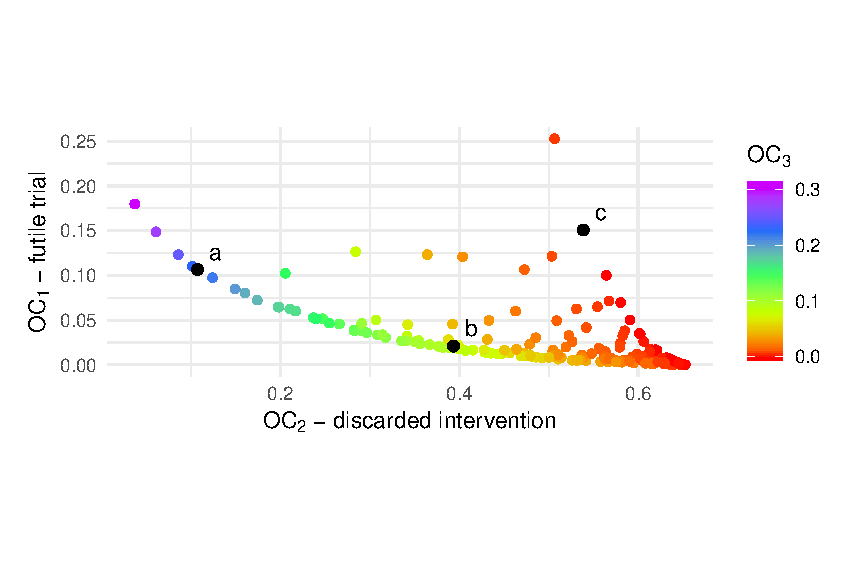
\includegraphics[scale=0.7]{./Figures/p_front}
\caption{Operating characteristics of efficient decision rules for the REACH trial with $k=12$ clusters.}
\label{fig:p_front}
\end{figure}

\begin{figure}
\centering
\includegraphics[scale=0.7]{./Figures/grid_p_front}
\caption{Operating characteristics of efficient decision rules for the REACH trial with $k=12$ clusters - a grid search, where grey solutions are dominated.}
\label{fig:grid_p_front}
\end{figure}

From Figure~\ref{fig:p_front} we immediately see the range of operating characteristics which are feasible, given the fixed sample size, and the trade-offs between these which we must consider. For example, the results suggest that we need not consider values of $OC_{1}$, $OC_{2}$, and $OC_{3}$ greater than 0.38, 0.44, and 0.56 respectively. Moreover, rules which reduce one of the operating characteristics to 0 are found for each case.

In the rules of the approximation set we see an almost linear inverse relationship between $OC_{2}$ and $OC_{3}$. To understand why this is, note that if we assume the term $p_{G,r}$ in $OC_{3}$ is approximately 0, we are left with $OC_{2} = p_{R,a} + p_{G,a}$ and $OC_{3} \approx p_{A,r} + p_{A,g}$. Thus, these criteria are almost opposite: $OC_{2}$ is the probability of incorrectly making the decision $a$; $OC_{3}$ is the probability of incorrectly \emph{not} making decision $a$. The larger the area corresponding to decision $a$ in the decision rule, the larger $OC_{2}$ and the smaller $OC_{3}$ will be. This is illustrated when comparing the decision rules labelled (a) and (b) in Figure~\ref{fig:p_front}, shown in Figures~\ref{fig:rule_a} and~\ref{fig:rule_b} respectively. The former rule achieves a low $OC_{3} \approx 0.025$ by having a relatively high threshold for making decision $r$. In contrast, rule (b) leads to decision $r$ more easily, resulting in higher $OC_{3}$.

\begin{figure}
\centering
\includegraphics[scale=0.7]{./Figures/dr_ex_a}
\caption{Example efficient decision rule $(a)$.}
\label{fig:rule_a}
\end{figure}

\begin{figure}
\centering
\includegraphics[scale=0.7]{./Figures/dr_ex_b}
\caption{Example efficient decision rule $(b)$.}
\label{fig:rule_b}
\end{figure}

While the opportunity to trade-off performance between $OC_{1}$ and $OC_{3}$ is clear, there appears to be limited opportunity to improve in either of these at the expense of an increase in $OC_{2}$. This is particularly so for rules leading to a $OC_{3}$ value of less than around 0.2. Rule (c) in Figure~\ref{fig:p_front} represents an opportunity to reduce $OC_{2}$ at the expense of one or both of $OC_{1}$ and $OC_{3}$. As illustrated in Figure~\ref{fig:rule_c}, this is achieved by having a relatively small area corresponding to decision $a$, allowing larger areas for decisions $r$ and $g$. 

\begin{figure}
\centering
\includegraphics[scale=0.7]{./Figures/dr_ex_c}
\caption{Example efficient decision rule $(c)$.}
\label{fig:rule_c}
\end{figure}

\section{Discussion}\label{sec:discussion}

%One example of an adaptive approach to assessing recruitment rates in an internal pilot~\cite{Hampson2017}.

%although it has been suggested that this limitation may be overcome by allowing a higher type I error rate than the typical 0.025 - 0.1~\cite{Lee2000}. 

The benefits brought by the Bayesian approach must be set against the challenges it brings, particularly in terms of computation time and operational feasibility. In terms of the latter, we are required to specify a joint prior distribution over the parameters $\theta$ and a partitioning of the parameter space into the three hypotheses. Moreover, a decision rule is also required if one does not wish to optimise over these. 

The specification of a joint prior distribution may be a particularly challenging and time-consuming task. Although some relevant data relating to similar parameters in different trials may be available, expert opinion will still be required to articulate the relevance of such data to the problem at hand. When no data at all are available, which is not unlikely given the early phase nature of pilot studies, expert opinion will be the only source of information. Elicitation of expert opinion can be conducted using an appropriate tool, such as the Sheffield Elicitation Framework (SHELF)~\cite{OHagan2006a}. The expense incurred through formal elicitation may make it hard to justify, particularly at the grant application stage. Where possible, the statistical model should be constructed with an aim to ensuring the parameters can be considered independent~\cite{OHagan2012}, thus allowing the full joint distribution to be defined as the product of the individual priors.  Although we used the same prior distribution when simulating the trial data and when conducting the Bayesian inference on that data in our examples, An alternative approach would be to use separate priors for each stage~\cite{Wang2002}. For example, it may be that for the analysis to be accepted as `objective', a vague or non-informative prior must be used at the analysis. Such a strategy is simple to carry out in the proposed method.

In addition to specifying priors, the parameter space must also be divided into three hypotheses. This may also prove challenging in practice, particularly when the number of parameters to be considered is greater than two. Further methodological research will be required to understand how best to elicit this information.

Although we have not described a fully decision-theoretic approach to the design and analysis of pilot trials, any decision rule of the form described in Section~\ref{sec:methods} may have an equivalent utility function such that using the rule will always lead to the same decision as maximising the utility function. For example, the decision rule illustrated in Section~\ref{fig:rule_simple} is equivalent to choosing $i \in \mathcal{D}$ such that $\mathbb{E}_{\phi}[u(i, \phi)]$ is maximised, where $u(i, \phi)$ is a discrete function taking values as given in Table~\ref{tab:utility}.

\begin{table}
\centering
\begin{tabular}{r r r r r}
\toprule
& & $\phi \in \Phi_{R}$ & $\phi \in \Phi_{A}$ & $\phi \in \Phi_{G}$ \\
\midrule
\multirow{3}{*}{Decision} & $r$ & - & - & - \\
 & $a$ & - & - & - \\
 & $g$ & - & - & - \\
\bottomrule
\end{tabular}
\caption{Latent utility function (to complete).}
\label{tab:utility}
\end{table}

The computational burden of the proposed method is significant, particularly when the model is too complex to allow a simple conjugate analysis to be used when sampling from the posterior distribution. One potential approach to improve efficiency is to use non-parametric regression to predict the result of a Bayesian inference, given some simulated data, thus bypassing the need to undertake a full MCMC analysis for each of the $N$ samples in Equation~\ref{eqn:MC_prob}. This approach has been applied successfully in the context of expected value of information calculations~\cite{Strong2014, Strong2015}. In terms of optimal design, we have not considered here the question of finding the smallest sample size such that leads to sufficient operating characteristics. The small samples typically available for pilot trials suggests that such optimisation may not be crucial. When it is deemed necessary, methods developed for the design and analysis of expensive computer experiments may provide a way for it to be conducted in an efficient manner~\cite{Jones2001}.

A number of modifications could be made to the proposed methodology. In particular, any operating characteristic could be defined and used in addition to, or instead of, the three proposed in this paper, providing they can be defined in terms of the probabilities of Table~\ref{tab:probs}. The multi-criteria optimisation methodology we have described will extend easily as the number of criteria are increased, although it should be noted that the presentation of solutions will become challenging.

Comparison with the frequentist approach. If we can get the WP1 paper published, we can take the same example and compare. Use a uniform prior over the frequentist hypothesis space?

Think about using independence ideas to help construct the hypotheses  - e.g. preference independence, where our preferences between $y$ and $y'$ doesn't change as $z$ changes to $z'$. That is not always the case here - it is something we have to assume in the frequentist case. But we can break the problem down using this - e.g. we might have trade-offs between follow-up and cluster size, and trade-offs between efficacy and adherence, but these two groups are preferentially independent from each other. 

Connection to multiple testing literature as discussed in WP1. \cite{Chuang-Stein2007} - Challenge of multiple co-primary endpoints: a new approach. Discusses the `reverse multiple testing problem', where we want all the endpoints to be good rather than any of them. Notes the problem with doing multiple univariate tests and proceeding if all are positive is that it can give low overall power. Argues that instead of controlling maximum type I error, we should control average type I error over the null space - so a kind of hybrid Bayesian approach. 

Our design considers the probability of making an amber decision when in the amber hypothesis. We do not consider what that decision will actually look like. For example, the type of amber adjustments needed are very different in different parts of the hypothesis, so we might end up adjusting recruitment and leaving adherence when it is the other way round, and our design does not consider that as an error. This points to a significant challenge in pilot trials - the difficulty in modelling post-trial action, the richness of the decision space. Contrast with the drug setting where nothing much changes, and we just decide on a phase III sample size. Hence plenty papers looking at optimising the whole process, not just the phase II trial itself.

%\item We have proposed three specific OCs, but we could define others. For example, we may be interested in the probability of choosing green, conditional on hypothesis $A$ being true. Note that, having calculated the probabilities of each mutually exclusive event, it would be easy to compute other OCs for a given design. We can include these in the multi-objective optimization over decision rules, although this will give a harder problem and we won't be able to plot the resulting Pareto front so easily. 

%\item The partitioning of the parameter space into three hypotheses may be challenging, particularly when we move beyond two dimensions. Iterative active learning algorithms which ask the user to label a set of points could help us define this partition empirically, although we would then need to consider the effect of uncertainty in the true partitioning and how this propagates through to the OC estimates. In two dimensions we could look at drawing the regions and then constructing a mathematical representation using a machine learning method, rather than defining the mathematical form and then drawing it. This may add an extra overhead to computation time if predicting fro the model is not very fast.

%\item The computational burden is significant for realistic problems. A potential approach to improving computational efficiency is through the construction of surrogate models / emulators.

%\item We have described optimising over decision rules, but could argue we should be able to define these a priori based on judgements other than the implied OCs, such as judgements about the relative cost of each type of error.

%\item We are automating MCMC Bayesian analyses here, and so cannot fully diagnose any problems with convergence.

%\item We do not consider optimising over the sample size. This makes some sense for pilot trials, where budget constraints mean they will never be very large (so not a large space to optimise over). Also want a large sample for other feasibility questions not incorporated into our design? But if we want to optimise, we can consider methods for efficient global optimisation of expensive computer code.

%\item We have considered hypotheses defined on the substantive parameter space, but could argue that nusiance parameters should be considered too. For example, we may not want to proceed if the ICC is so high that a phase III trial would not be feasible. A different framework, where we model the phase III trial and define appropriate assurance measures, might address these issues better.

%\item Each decision rule is associated with a latent, implied utility function, where doing MEU would lead to the same decisions. Such a function won't necessarily be unique. This is just what we had earlier when we used LP to find a stepwise function with expectation maximised over the relevant area. Give an example - it may motivate a fully decision-theoretic approach if it is disagreeable in some way.

\bibliographystyle{plain}
\bibliography{U:/Literature/Databases/DTWrefs}

\end{document}

%A simple Monte Carlo estimate is then
%\begin{equation} \label{eqn:MC_prob}
%p_{i,j} \approx \frac{1}{N_{out}} \sum_{k=1}^{N_{out}} I(\phi^{(k)} \in \Phi_{i}, a(x^{(k)}) = j),
%\end{equation}
%where the $\phi^{(k)}, x^{(k)}$ are simulated from the joint prior distribution $p(\phi, x) = p(x \mid \phi)p(\phi)$. For each sample we compute $a(x^{(k)})$, which %requires calculating the posterior probabilities $p_{R}^{(k)}, p_{G}^{(k)}$. Given $N_{in}$ samples $\phi^{(m)}$ from the posterior distribution $p(\phi \mid x^{(k)})$, %these can be approximated by
%\begin{align}
%p_{i}^{(k)} \mid x &= \mathbb{E}_{\phi \mid x^{(k)}} [ I(\phi \in \Phi_{i}) ] \\
% & \approx \frac{1}{N_{in}} \sum_{m=1}^{N_{in}} I(\phi^{(m)} \in \Phi_{i}).
%\end{align}

Estimation of the probabilities in Table~\ref{tab:probs} can be done under a Bayesian framework. That is, rather than focussing on point estimates and their standard errors / confidence intervals, we instead infer a distribution on the probability vector $\xi$ which fully describes our knowledge and uncertainty in it. Specifically, we consider the $(h(\phi), d)$ outcome of the trial to follow a multinomial distribution under $n=1$ and $\xi$. Consider the following process:
\begin{enumerate}
\item sample $(\phi, x) \sim p(\phi, x)$
\item generate $N_{i}$ samples $\phi \sim p(\phi | x)$
\item assuming $\eta \sim p(\eta) = Dir(1)$ and $h(\phi | x) \sim MN(N_{i}, \eta)$, we have $p(\eta | \phi, x) = Dir(h(\phi | x))$
\item choose decision using $a(\hat{\eta})$, where $\hat{\eta} = (\frac{h(\phi | x)_{1}}{N_{i}} , \ldots , \frac{h(\phi | x)_{9}}{N_{9}})$
\item report the hypothesis-decision pair $(h,d)$
\end{enumerate}
The above process simulates an outcome of the pilot trial, including the true values of the model parameters, the data obtained, the posterior inference, and the subsequent decision made. Repeating the process $N_{o}$ times gives us an instance of the random variable $c \sim MN(N_{o}, \xi)$. Assuming a flat Dirichlet prior for $\xi$, the posterior distribution given the simulated data $c$ is then $\xi \sim Dir(c+1)$.

In step (4) of the above process, the decision made is based on the expectation of the posterior probability vector $\eta$. If this is indeed how decisions are to be made in practice, the above method is sound (we may have to assume that the same seed is used for the inner MCMC sampling). However, we might expect that in practice we will want to use some $N_{i}^{*} \gg N_{i}$ when sampling from the posterior $p(\eta | \phi, x)$ to obtain a more highly concentrated distribution $p(\eta | \phi, x)$, and therefore minimise the chance that $a(\hat{\eta}) \neq a( \mathbb{E}_{\eta | \phi, x}[\eta] )$. In this case, the above process is an approximation of what will happen. In particular, at stage (4), when we use some very large $N_{i}^{*}$ we will obtain the (almost) true $\mathbb{E}_{\eta | \phi, x}[\eta]$.

% First, outline exactly how we will analyse the data to make a decision
The posterior probabilities (which we will now refer to as $\eta = (p_{R}, p_{A}, p_{G})$ referred to above will be estimated by generating $N_{i}$ samples from the posterior distribution $\phi \sim p(\phi | x)$ (probably using MCMC). The number of times a posterior sample $\phi$ is located in region $\Phi_{i}$ is recorded for $i = R, A, G$. We denote the vector of counts of such instances by $c$. We can then model belief about the true posterior probabilities $\eta$ using a multinomial-Dirichlet conjugate model, where $c \sim MN(N_{i}, \eta)$, prior $\eta \sim p(\eta) = Dir(1)$, and so $\eta | c \sim p(\eta | c) = Dir(c+1)$. The decision taken is $a(\hat{\eta})$, where $\hat{\eta} = \mathbb{E}_{\eta | c}[\eta]$.

To inform the distribution of $\xi$ we can simply simulate $N_{o}$ instances of $(h, d)$ events:
\begin{enumerate}
\item sample $(\phi, x) \sim p(\phi, x)$
\item generate $N_{i}$ samples $\phi \sim p(\phi | x)$
\item assuming $\eta \sim p(\eta) = Dir(1)$ and $h(\phi | x) \sim MN(N_{i}, \eta)$, we have $p(\eta | \phi, x) = Dir(h(\phi | x))$
\item choose decision using $a(\hat{\eta})$, where $\hat{\eta} = \mathbb{E}_{\eta | c}[\eta]$
\item report the hypothesis-decision pair $(h,d)$
\end{enumerate}
This gives a nine-dimensional count vector $e$ following a multinomial distribution with $n=N_{o}$ and probability vector $\xi$, so we can update $p(\xi)$ given this simulated data to give our posterior distribution of the probability vector $\xi$. This distribution can then be used to calculate any expectations or variances for the individual probabilities or their combinations as operating characteristics.


%%%%%%%%%%%%%%%%%%%%%%%%%%%%%%%%%%%%

Back to efficient calculation methods. We had previously focussed on finding a shortcut for estimating posterior probabilities using non-parametric regression, so that these can be used to get decisions directly from data via the decision rule. Can we bypass the posterior-based decision rule entirely? Can we use simulated data to define the decision rule as an acceptance region, and then assess its properties? For example, we can do the model fitting we have worked out before but instead of worrying about how accurate it is, we can use it as a guide to find a rule / acceptance region but then assess its actual properties.

Difficulty here is that we are proposing a trial analysis that compares data with an acceptance region based on summary stats - not Bayesian at all. And the acceptance region is likely to be very complex and idiosyncratic. But we have optimised over Bayesian decision rules to give the desired unconditional operating characteristics - is this right? From a Bayesian perspective, we only care about the data obtained. The inference concerns only the data, but it is the decision we are focussed on - how we go from the inference to the decision. So is this really a utility issue? Again, given the utility function we do not need to pre-specify a decision rule - it falls out automatically from the MEU method. So are we effectively defining a latent utility function that gives us the desired OCs when we optimise over posterior decision rules? Yes - exactly this. Can argue that we shouldn't, that utility should be defined on its own. But OCs certainly interesting, e.g. from a sensitivity point of view.

%%%%%%%%%%%%%%%%%%%%%%%%%%%%%%%%%%%%%



